\documentclass{report}
\usepackage[T1]{fontenc} % Fontes T1
\usepackage[utf8]{inputenc} % Input UTF8
\usepackage[backend=biber, style=ieee]{biblatex} % para usar bibliografia
\usepackage{csquotes}
\usepackage[portuguese]{babel} %Usar língua portuguesa
\usepackage{blindtext} % Gerar texto automaticamente
\usepackage[printonlyused]{acronym}
\usepackage{hyperref} % para autoref
\usepackage{graphicx}

\bibliography{bibliografia}


\begin{document}
%%
% Definições
%
\def\titulo{EVOLUÇÃO TECNOLÓGICA}
\def\data{28/11/2019}
\def\autores{Rafael Santos, André Alves}
\def\autorescontactos{(98466) rafaelmsantos@ua.pt, (94190) afla@ua.pt}

\def\departamento{DEPARTAMENTO DE ELETRÓNICA E TELECOMUNICAÇÕES}
%\def\empresa{EMPRESA}

\def\logotipo{ua.pdf}
%
%%%%%% CAPA %%%%%%
%
\begin{titlepage}

\begin{center}
%
\vspace*{50mm}
%
{\Huge \titulo}\\ 
%
\vspace{10mm}
%
%{\Large \empresa}\\
%
\vspace{10mm}
%
{\LARGE \autores}\\ 
%
\vspace{30mm}
%
\begin{figure}[h]
\center
\includegraphics{\logotipo}
\end{figure}
%
\vspace{30mm}
\end{center}
%
\begin{flushright}
%\versao
\end{flushright}
\end{titlepage}

%%  Página de Título %%
\title{%
{\Huge\textbf{\titulo}}\\
{\Large \departamento\\ }
}
%
\author{%
    \autores \\
    \autorescontactos
}
%
\date{\data}
%
\maketitle

\pagenumbering{roman}

%%%%%% RESUMO %%%%%%
\begin{abstract}

\end{abstract}

%%%%%% Agradecimentos %%%%%%
% Segundo glisc deveria aparecer após conclusão...
%\renewcommand{\abstractname}{Agradecimentos}
%\begin{abstract}
%Eventuais agradecimentos.
%Comentar bloco caso não existam agradecimentos a fazer.
%\end{abstract}


\tableofcontents
% \listoftables     % descomentar se necessário
% \listoffigures    % descomentar se necessário


%%%%%%%%%%%%%%%%%%%%%%%%%%%%%%%
\clearpage
\pagenumbering{arabic}

%%%%%%%%%%%%%%%%%%%%%%%%%%%%%%%%
\chapter{Introdução}
\label{chap.introducao}

Neste trabalho iremos abordar a evolução tecnológica através da exposição e explicação de várias invenções que ditaram a evolução do mundo onde vivemos hoje. Iremos também falar dos seus inventores.
Foi nos proposto ser realizado este trabalho para a cadeira de Laboratórios de Informática, onde decidimos escolher este tema pois entendemos ser interessante, enriquecendo também a nossa cultura geral.  


\chapter{Invenção da Máquina de Imprensa}

A máquina de imprensa foi inventada em 1439 pelo alemão Johann Gutenberg. Nasceu em Mainz na Alemanha em 1395 e morreu em 1468.Foi Serralheiro (especialista no trabalho do ouro e outros materiais preciosos) e o inventor da máquina de imprensa.

A imprensa de Gutenberg foi desenvolvida a partir da confeção e combinação de tipos móveis (símbolos gráficos moldados em chumbo) que eram passados em tinta à base de óleo de linhaça e impressos em papel por meio de uma prensa movimentada por uma barra de madeira.

Deve-se ter em atenção que Gutenberg não inventou a imprensa, visto que este processo já era conhecido na China.Mas Gutenberg aperfeiçoou os métodos de divulgação por meio da criação da prensa e dos tipos móveis e iiso sim foi o que tornou a sua invenção inovadora. Até 1489 as prensas idênticas à de Gutenberg já estariam espalhadas pela Europa mais propriamente Espanha, França, Holanda, Inglaterra e Dinamarca. No ano de 1500 já haviam sido produzidos cerca de 15 milhões de documentos. 

O primeiro livro a ser impresso com a utilização do método de tipos móveis inventado por Gutenberg foi a Bíblia. A impressão da Bíblia é considerada um momento revolucionário da história Humana, permitindo a popularização do conhecimento. Foram impressos 180 exemplares, mas apenas estão guardados 49 exemplares em vários museus, estando um deles na cidade Natal do inventor, Mainz.
 \pagebreak
A melhoria do processo foi considerada uma mais valia pois para além da Bíblia outros documentos (tal como as cartas de indulgência que eram recebidas pelos fiéis após o pagamento para o livramento de penas e até mesmo do purgatório) poderiam ser impressos em maior quantidade. 
Esta invenção permitiu que em vários centros urbanos da Europa fossem criados mais máquina impulsionando assim a produção em grandes quantidades de todos os tipos de documentação desde livros,panfletos,etc.


\begin{center}
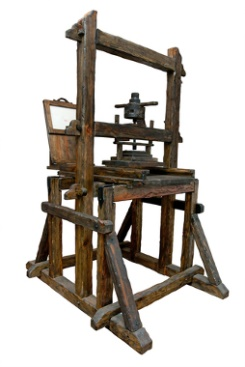
\includegraphics[height=6cm,width=5cm]{artigo/mp}
\end{center}
 \begin{figure}[h]
 	\centerline{\fbox{Fig.1-Máquina de Imprensa.}}
 \end{figure}








\chapter{Invenção do microscópio}
%\label{chap.resultados}
%Descreve os resultados obtidos.

Nascido em 1580 e falecido em 1638 (58 anos) ,Zacharias Janssen foi um inventor Holandês tendo inventado o microscópio em 1590 .
Como seria um homem ainda muito jovem há quem acredite que Janssen teve ajudo do seu pai pois este seria um fabricante de lentes.

Esta invenção mudou a perspetiva do Homem em relação ao mundo, possibilitando a observação e exploração de várias áreas que até aquela altura seriam desconhecidas, revolucionando e atualizando assim o conhecimento científico. Com esta invenção foi-nos possível ver tudo aquilo que a olho nu nos seria impossível.

Esta invenção provocou o desabamento de várias teorias (como por exemplo a da geração espontânea (onde se acreditava que os organismos vivos podem-se originar de matéria inanimada) 
Possibilitou também a descoberta da origem de doenças, que até à altura se pensava que seriam originadas pelo sobrenatural, visto que possibilitou a visão e análise das criaturas microscópicas que as originavam.


\begin{center}
\ 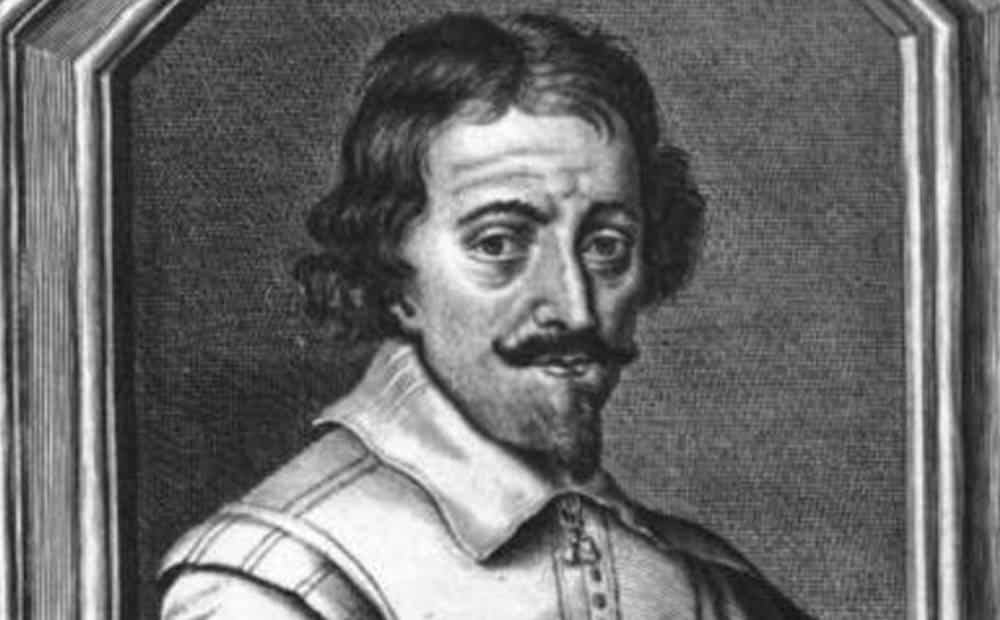
\includegraphics[height=5cm,width=5cm]{artigo/janssen}
\end{center}
 \begin{figure}[h]
 	\centerline{\fbox{Fig.2-Zacharias Janssen.}}
 \end{figure}

\pagebreak
A palavra microscópio tem origem nos termos mikrós (pequeno) e scoppéo (Ver, observar).

Atualmente os microscópios dividem se em duas categorias:
\begin{itemize}
	\item Microscópio ótico: Funciona utilizando um conjunto de lentes: ocular e objetiva (lentes que posicionadas de determinada forma conseguem corrigir deformações cromáticas) que ampliam a imagem transpassada por um feixe de luz.Possui uma parte ótica,onde a imagem é ampliada, e uma parte mecânica, que atua como suporte do sistema ótico ajudando na questão da focagem da imagem.
	\item Microscópio eletrónico: Amplia a imagem utilizando feixes de eletrões. Não há lentes de cristal mas sim bobinas,que têm o nome de lentes eletromagnéticas.
\end{itemize}

\begin{center}
\ 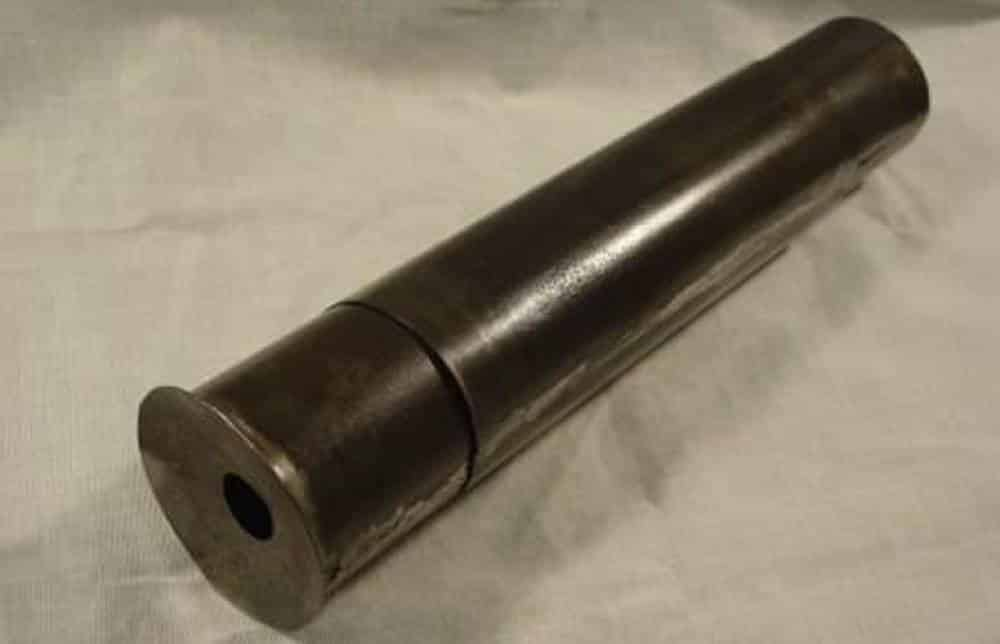
\includegraphics[height=4cm,width=4cm]{artigo/microscopio}
\end{center}
 \begin{figure}[h]
 	\centerline{\fbox{Fig.3-Microscópio.}}
 \end{figure}
 
 
 

\chapter{Invenção do motor a vapor}
\label{chap.analise}
%Analisa os resultados.
O motor a vapor foi inventado por Thomas Newcomen em 1712 muitas vezes chamada por Máquina Atmosférica de Newcomen. O motor é operado pelo vapor de condensação introduzido no cilindro criando assim um vácuo parcial, permitindo que a pressão atmosférica empurre o pistão para dentro do cilindro.

Foi o primeiro dispositivo prático a utilizar o vapor para produzir trabalho mecânico. 

James Watt nasceu a 19 de Janeiro de 1736 em Greenock, na Escócia e faleceu em 1819 a 25 de Agosto em Heathfield Hall,Inglaterra.

Em 1763, recebeu para arranjar uma máquina a vapor, a de Newcomen, que era a mais avançada da altura. No processo de arranjo reparou que conseguia melhor o seu rendimento. Primeiro era necessário elevar a temperatura do vapor, arrefecendo-o depois bruscamente durante a expansão. Decidiu também acrescentar outros artifícios, como por exemplo um condensador de vapor, criando assim uma verdadeira máquina a vapor cujo rendimento seria 75\% mais elevado do que a máquina de Newcomen.

Esta máquina deu origem à primeira patente registada por James Watt em 1769.
Entre 1776 e 1781 andou a viajar por todo o Reino Unido a instalar as suas máquinas fazendo também várias melhorias e modificações, sendo que algumas delas facilitaram a sua instalação. 

\begin{center}
\ 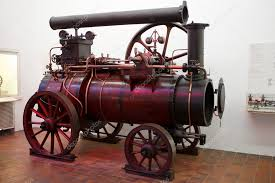
\includegraphics[height=3cm,width=4cm]{artigo/motorvapor}
\end{center}
 \begin{figure}[h]
 	\centerline{\fbox{Fig.4-Motor a vapor.}}
 \end{figure}


\chapter{Invenção da bateria elétrica}
\label{chap.conclusao}
%Apresenta conclusões.

O crédito pela invenção da bateria elétrica é dado ao cientista Alessandro Volta.

Alessandro Volta nasceu em Itália a 18 de fevereiro de 1745 e faleceu a 5 de março de 1827, tendo sido durante os seus 82 anos um dos grandes físicos do século XVIII. Foi o criador da pilha e provou que o seu amigo Luigi Galvani estaria errado ao dizer que a corrente elétrica só seria gerada por seres vivos;

Foi mesmo devido a essa discordância entres os dois que surgiu a “necessidade” de provar o contrário ao seu amigo. Volta determinou que os melhores pares de metais dissimilares para a produção de eletricidade eram o zinco e a prata e que ,se estes fossem colocados em certas soluções químicas, ocorreria a produção de eletricidade.

Decidiu colocar camadas de zinco e cobre juntos e alternadamente com pedaços de papelão embebidos em Salmoura. O arco metálico condutor foi utilizado para transportar a eletricidade a uma distância maior. A pilha de volta (pilha Voltiac) foi a primeira pilha a produzir uma corrente ,de forma estável, de eletricidade.

\begin{center}
\ 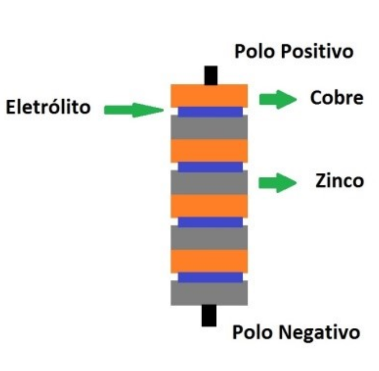
\includegraphics[height=4cm,width=4cm]{artigo/bateria}
\end{center}
 \begin{figure}[h]
 	\centerline{\fbox{Fig.5-Bateria.}}
 \end{figure}


\chapter{Invenção da fotografia}
 Joseph Nicéphore Niépce nasceu a 7 de Março de 1765 em Saône-et-Loire e morreu a 5 de Julho de 1833 também em Saône-et-Loire. 
 
 Foi um inventor Francês e o grande responsável por uma das primeiras fotografias. Ele conseguiu fazer com que as fotografias não desaparecessem em 1826 chamando a esse processo de heliografia (processo esse que demoraria cerca de oito horas para gravar a imagem.)

A tecnologia que levou à invenção da fotografia junta duas ciências distintas: ótica (convergência de raios de luz para formar uma imagem dentro da câmara) e química ( para permitir que essa imagem seja capturada e gravada permanentemente numa superfície fotossensível, ou seja a fotografia não é nada mais do que luz impressa sobre uma película. 

A palavra “fotografia” significa literalmente “desenhar com luz”.
Uma câmara fotográfica é basicamente uma caixa escura, com um orifício para entrar luz e com uma superfície sensível à luz.
A fotografia é o processo de criação de imagens por meio de exposição luminosa e reações químicas fixando-as numa superfície sensível.

Foi no ano de 1826 que foi reconhecida a primeira fotografia e foi atribuída ao francês Joseph Nicéphore Niépce. No entanto não é obra de um só autor, mas sim de um processo de vários avanços por parte de vários autores que trabalharam juntas e durante longos anos.
\begin{center}
\ 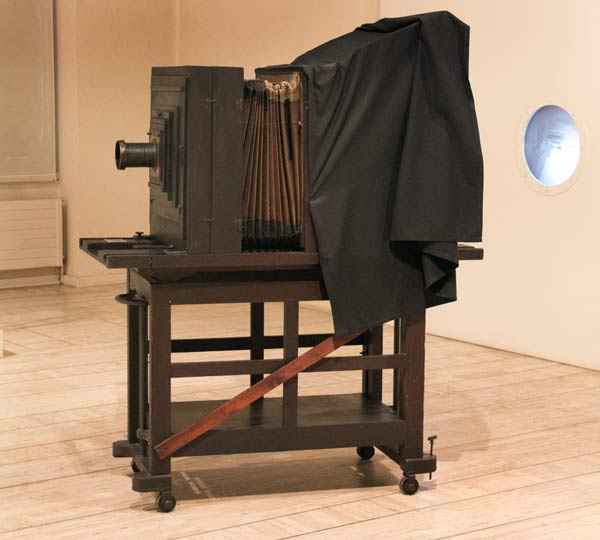
\includegraphics[height=3cm,width=3cm]{artigo/fotografia}
\end{center}
 \begin{figure}[h]
 	\centerline{\fbox{Fig.6-Primeira máquina fotográfica.}}
 \end{figure}

\pagebreak

Alguns anos depois, Nièpce entrou em parceria com Louis Daguerre e juntos melhoraram o processo substituindo por uma resina mais sensível à luz e melhorando o tratamento pós-exposição. 

Desde então, o processo de evolução da fotografia e das próprias câmaras não tem parado. O formato digital e vídeo são algo bastente comum nas sociedades industrializadas ,cada vez com mais qualidade e cada vez mais funcionalidades sendo também, em termos monetários mais acessíveis .

Desde o tempo de Nièpce onde havia dificuldades em obter de forma fixa uma simples imagem até aos tempos modernos de hoje pode-se ver a grande evolução que a fotografia teve ,estando até a um simples passo de nós através de um simples clique na tela do nosso telemóvel.

\begin{center}
\ 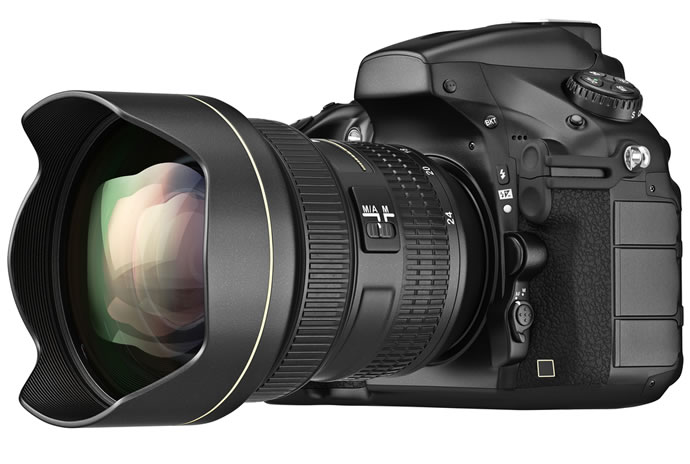
\includegraphics[height=5cm,width=7cm]{artigo/camara}
\end{center}
 \begin{figure}[h]
 	\centerline{\fbox{Fig.7-Máquina fotográfica moderna.}}
 \end{figure}


\chapter{Invenção do motor a combustão}
O crédito da criação do motor a combustão foi atribuído a Nikolaus August Otto. A sua invenção revolucionou a indústria visto que na altura apenas existiam e eram utilizados os motores a vapor. Ele foi o desenvolvedor do chamado de Ciclo de 

Otto que é constituído por quatro partes.
-A admissão: A chamada câmara de combustão para onde entra o combustível e ar.
- Compressão da câmara;
-Explosão: liberta-se uma faísca no seu interior provocando uma ignição que expande a câmara de combustão;
-Escape: os gases formados na combustão são expelidos e as válvulas para entrada de arr e combustível são abertas reiniciando o processo.
	Todo este processo combinado com um sistema de transmissão define o que se chama motor de combustão interna.
\begin{center}
\ 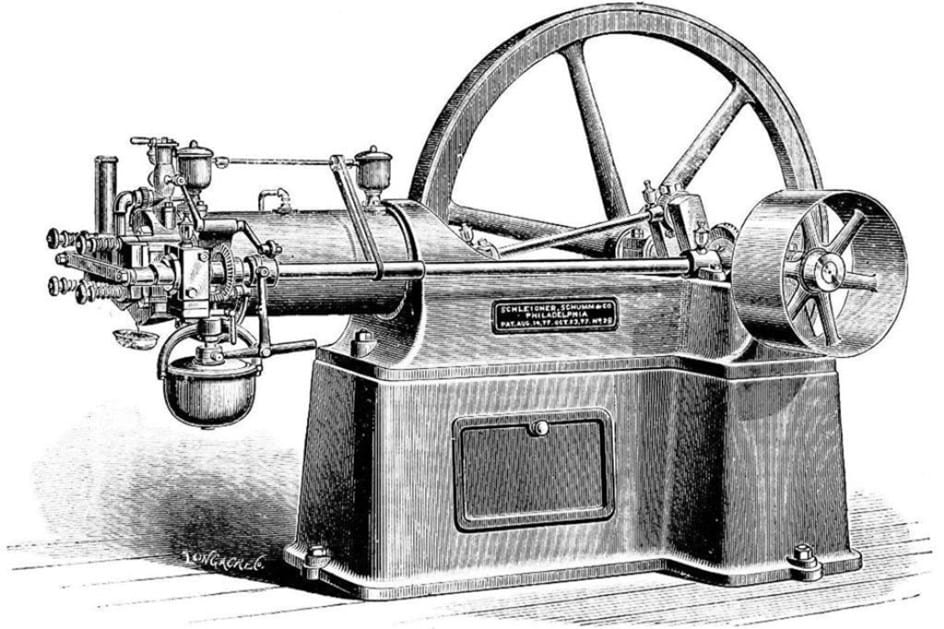
\includegraphics[height=5cm,width=5cm]{artigo/otto}
\end{center}
 \begin{figure}[h]
 	\centerline{\fbox{Fig.8-Motor de combustão de Otto.}}
 \end{figure}

\pagebreak
Geralmente, um motor atual possui os seguintes componentes:
-Componentes fixos:
\begin{itemize}

\item O bloco, estrutura que sustenta os cilindros e o eixo de transmissão;
\item O cárter, que assegura a lubrificação das peças do motor;
\item A cabeça do motor ,onde se encontram as velas de ignição e as válvulas;
Componentes moveis:
\item a cambota, que transforma o movimento linear do pistão em circular;
\item o pistão, que se move dentro do cilindro definindo o volume da câmara de combustão;
\item a biela, que liga o pistão à cambota;
\end{itemize}

Nikolaus August Otto nasceu a 10 de junho de 1832 na Alemanha e morreu a 26 de janeiro de 1891, tendo morrido com 58 anos.

\begin{center}
\ 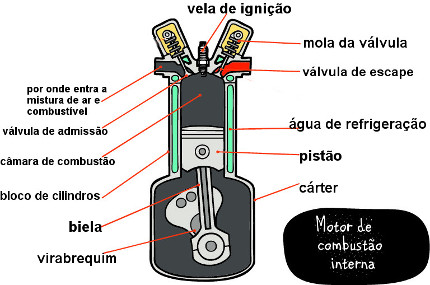
\includegraphics[height=5cm,width=5cm]{artigo/otto2}
\end{center}
 \begin{figure}[h]
 	\centerline{\fbox{Fig.9-Motor a combustão.}}
 \end{figure}

\chapter{Invenção do automóvel}
Antes do automóvel as pessoas moviam-se a pé, por meio de carruagens, cavalos e carroças. Devido à necessidade de se criar uma maneia de locomoção mais rápida e, portanto, mais eficiente surgiu assim a ideia do automóvel.

O primeiro automóvel foi criado por Karl Friedrich Benz em 1886.
Benz era um engenheiro mecânico que nasceu na Alemanha e que patenteou o carro de 3 rodas com o seu próprio sistema de acelerador, velas de ignição, engrenagens, radiador de água, carburador e vários outros componentes.

Benz patenteou, mas não foi o primeiro a pensar na ideia. No entanto a ideia de Benz foi a única que saiu do papel e que funcionou.

Após várias tentativas com resultado negativo, karl Benz conseguiu desenvolver um carro prático comum que era constituído por motor de combustão interno e que era movido a gasolina, servindo assim de modelo para os carros que possuímos hoje em dia.

Benz nasceu em 1844 na Alemanha, em Karlsruhe. Quarenta anos mais tarde morreu não tendo hipótese de constatar o sucesso e importância que a sua invenção teria.
No entanto, 2 anos antes da sua morte Benz juntou-se à empresa automóvel do colega Gottlieb Daimler tendo assim formado o grupo Daimler, o fabricante da marca automóvel Mercedes-Benz.

\begin{center}
\ 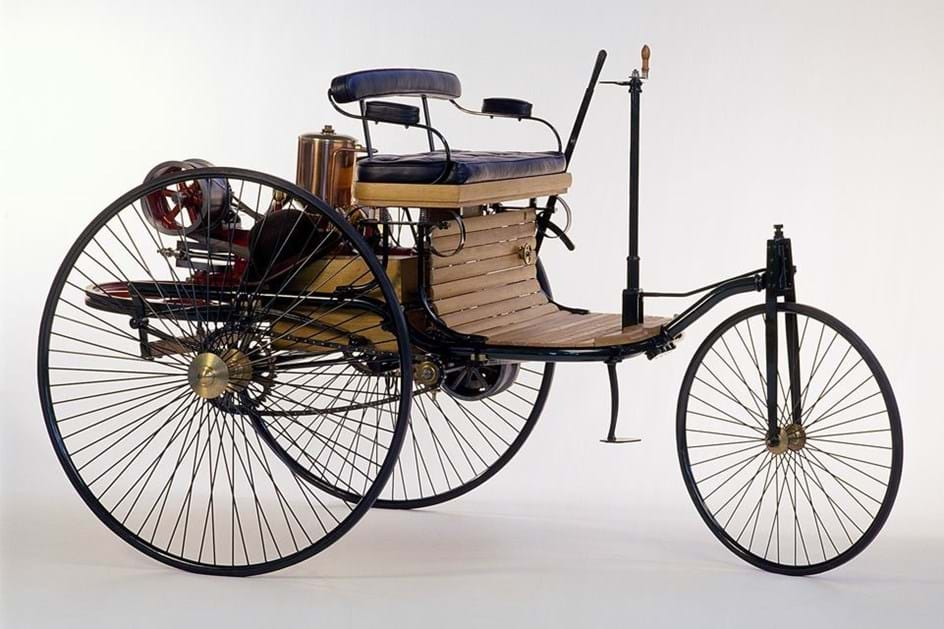
\includegraphics[height=3cm,width=4cm]{artigo/Benz}
\end{center}
 \begin{figure}[h]
 	\centerline{\fbox{Fig.10-Primeiro automóvel.}}
 \end{figure}

\chapter{Invenção do avião}
O surgimento do avião foi uma das maiores evoluções tecnológicas. A sua invenção fez com que o tempo de viagens entre duas cidades, quer no mesmo país, quer em países diferentes diminuísse de forma significativa.

O avião propriamente dito foi criado no início do século XX. Mas agora  entra uma das maiores polémicas da história: quem será o inventor? Os irmãos Wright ou o brasileiro Santos Dumont?

Em 1903, os irmãos Wright conseguiram pôr o avião no ar, mas com a ajuda de uma catapulta, não tendo testemunhas credíveis sobre o acontecimento.

\begin{center}
\ 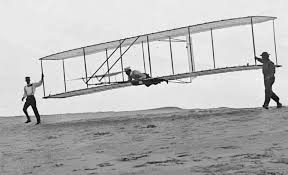
\includegraphics[height=5cm,width=5cm]{artigo/aviaowright}
\end{center}
 \begin{figure}[h]
 	\centerline{\fbox{Fig.11-Avião dos irmãos Wright.}}
 \end{figure}

\pagebreak

Mais tarde Santos Dumont voou sobre paris com o seu avião sem auxílio de nenhum instrumento, evento este que foi testemunhado pelos moradores da capital francesa e da imprensa local.
Muitos críticos argumentam sobre a invenção dos irmãos Wright dizendo que estes, devido ao facto de ser necessário o avião ser catapultado, não se pode considerar um avião. Outros dizem que o mais importante é voar e não o modo como é iniciado o voo. 

\begin{center}
\ 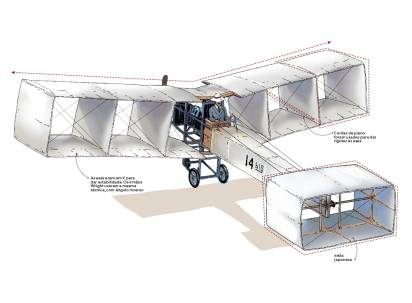
\includegraphics[height=5cm,width=5cm]{artigo/aviaosantos}
\end{center}
 \begin{figure}[h]
 	\centerline{\fbox{Fig.12-Avião de Santos Dumont.}}
 \end{figure}





\chapter{Invenção do computador}
Alan Turing é considerado o pai da computação. Foi ele um dos primeiros a pensar na ideia de ser possível uma máquina tornar-se inteligente.
Alan Turing nasceu a junho de 1912 em Londres e faleceu em junho de 1954, 42 anos.

O seu sucesso começou na altura da segunda guerra mundial ao trabalhar para a inteligência britânica. O matemático desenvolveu o chamado “Bombe” que traduziria os textos secretos dos alemães gerados por uma máquina intitulada de enigma. A “bombe” traduziria as mensagens da Enigma e transformava-as em mensagens credíveis e compreensíveis.

Alan Turing foi também nos primeiros a pensar na inteligência artificial ao querer verificar se o computador, ao serem-lhe enviadas perguntas, conseguiria distinguir se elas teriam sido feitas por uma pessoa ou uma máquina.
\begin{center}
\ 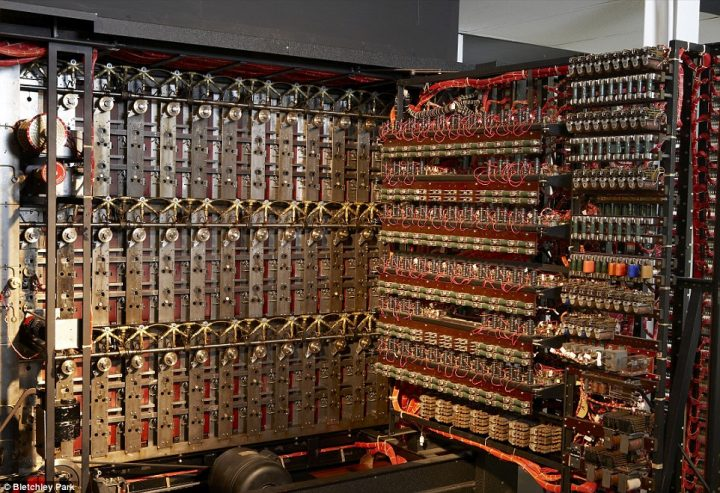
\includegraphics[height=5cm,width=5cm]{artigo/turing}
\end{center}
 \begin{figure}[h]
 	\centerline{\fbox{Fig.13-Computador de Turing.}}
 \end{figure}

  



\chapter*{Contribuições dos autores}
O Rafael fez os capítulos 2 a 10.
O André fez os capítulos 11 a 18.
O resto do trabalho foi feito em conjunto,considerando assim que o trabalho foi bem dividido com 50\%

%%%%%%%%%%%%%%%%%%%%%%%%%%%%%%%%%
\chapter*{Acrónimos}
\begin{acronym}
\acro{ua}[UA]{Universidade de Aveiro}
\acro{miect}[MIECT]{Mestrado Integrado em Engenharia de Computadores e Telemática}
\acro{lei}[LEI]{Licenciatura em Engenharia Informática}
\acro{glisc}[GLISC]{Grey Literature International Steering Committee}
\end{acronym}


%%%%%%%%%%%%%%%%%%%%%%%%%%%%%%%%%
\chapter{Bibliografia}

\printbibliography

\href {https://pt.wikipedia.org/wiki/Ficheiro:User-FastFission-brain.gif}{https://pt.wikipedia.org/wiki/Ficheiro:User-FastFission-brain.gif}

\href {https://pt.wikipedia.org/wiki/Imagem_por_resson\%C3\%A2ncia_magn\%C3\%A9tica}{link : ressonância magnética}

\href {https://pt.wikipedia.org/wiki/Reprodutor_de_DVD}{https://pt.wikipedia.org/wiki/ReprodutordeDVD}

\href {https://pt.wikipedia.org/wiki/Airbag}{https://pt.wikipedia.org/wiki/Airba}

\href {https://pt.wikipedia.org/wiki/Google}{https://pt.wikipedia.org/wiki/Google}

\href {https://pt.wikipedia.org/wiki/USB_flash_drive}{https://pt.wikipedia.org/wiki/USBflashdrive}

\href {https://www.uol/tecnologia/especiais/a-evolucao-do-iphone.htm#imagem-1}{https://www.uol/tecnologia/especiais/a-evolucao-do-iphone.htmimagem-1}

\href {https://brasilescola.uol.com.br/historiag/invencao-imprensa.htm}{https://brasilescola.uol.com.br/historiag/invencao-imprensa.htm}

\href{https://www.infoescola.com/termodinamica/motor-a-vapor/}{https://www.infoescola.com/termodinamica/motor-a-vapor/}

\href{https://kasvi.com.br/microscopio-microscopia-historia-evolucao/}{https://kasvi.com.br/microscopio-microscopia-historia-evolucao/}

\href{http://www.sta-eletronica.com.br/artigos/baterias-em-geral/informacoes-basicas/a-historia-das-baterias}{http://www.sta-eletronica.com.br/artigos/baterias-em-geral/informacoes-basicas/a-historia-das-baterias}

\href{https://www.infoescola.com/artes/fotografia/}{https://www.infoescola.com/artes/fotografia/}

\href{https://fluxoconsultoria.poli.ufrj.br/blog/projetos-mecanicos/motor-a-combustao/}[{https://fluxoconsultoria.poli.ufrj.br/blog/projetos-mecanicos/motor-a-combustao/}

\href{https://mundoeducacao.bol.uol.com.br/fisica/como-surgiu-aviao.htm}{https://mundoeducacao.bol.uol.com.br/fisica/como-surgiu-aviao.htm}

\href{https://comprasegura.standvirtual.com/historia-automovel/}{https://comprasegura.standvirtual.com/historia-automovel/}



\end{document}
